\documentclass{iacrtrans}
\usepackage[utf8]{inputenc}

% -- Better auto-referencing --
\usepackage{hyperref}
\usepackage[nameinlink]{cleveref}
\crefname{algocf}{alg.}{algs.}
\Crefname{algocf}{Algorithm}{Algorithms}

% -- Some neat table packages --
\usepackage{makecell}
\usepackage{arydshln}
\usepackage{siunitx} % For group separators when writing long integers

% -- Algorithms --
\usepackage[
    titlenumbered,
    linesnumbered,
    ruled
]{algorithm2e}
\SetKwInOut{Input}{Input}
\SetKwInOut{Output}{Output}
\SetKwInOut{Return}{Return}

\SetKwComment{Comment}{/* }{ */}
\newcommand\mycommentstyle[1]{\footnotesize\ttfamily\textcolor{red!70!black}{#1}}
\SetCommentSty{mycommentstyle}

% -- Setting format for equations --
\usepackage{xcolor}
\usepackage{empheq}
\usepackage{bbm}

\usepackage[most]{tcolorbox}

\newtcolorbox{empheqboxed}{%
  enhanced,
  boxsep=1pt,
  arc=0.75ex,
  colback=gray!10,
  colframe=gray!40,
  boxrule=1pt,
  leftrule=40pt,
  top=-3.5mm,
  overlay unbroken and first ={%
    \node[minimum width=1cm,
          anchor=south,
          font=\sffamily\bfseries,
          xshift=20pt,
          yshift=-6.5pt,
          black]
    at (frame.west) {Stack:};
  }
}

\usepackage[cache=false]{minted}
\usemintedstyle{tango}

% -- Bitcoin Script Commands --
\newcommand{\elem}[1]{\, \langle #1 \rangle \,}
\newcommand{\opcode}[1]{\, \texttt{#1} \,}
\newcommand{\script}[1]{ $\big\{ #1 \big\}$ }

\author{Dmytro Zakharov\inst{1}}
\institute{V.N. Karazin Kharkiv National University \email{zakharov2025mp11@student.karazin.ua}}
\title[Activation-Efficient Neural Networks]{Activation-Efficient Neural Network Architectures}

\begin{document}

\maketitle

% use optional argument because the \LaTeX command breaks the PDF keywords
\keywords[]{Neural Networks, Activation Functions, Architecture Optimizations, Zero-Knowledge, Fully Homomorphic Encryption}

\begin{abstract}
    Due to the rise of neural network architectures, the need for their privacy
    and privacy-preserving computations became paramount. For that reason, the 
    fields of zero-knowledge proofs and fully homomorphic encryption have been
    actively researched to work on top of neural networks. However, the 
    activation functions used in neural networks are not always compatible with
    the existing arithmetizations of cryptographic primitives. In this paper, we
    analyze whether the activation functions used in neural networks can be
    optimized for the sake of making them more ``cryptographically friendly''.
\end{abstract}

\tableofcontents{}

\section{Introduction}

Undeniably, the neural networks have become the cornerstone of modern machine
learning and artificial intelligence. They are used in almost every field of
computer science, from computer vision \cite{nns-in-cv-1,nns-in-cv-2} to natural
language processing \cite{nns-in-nlps-1,nns-in-nlps-2}.

\begin{figure}
    \centering
    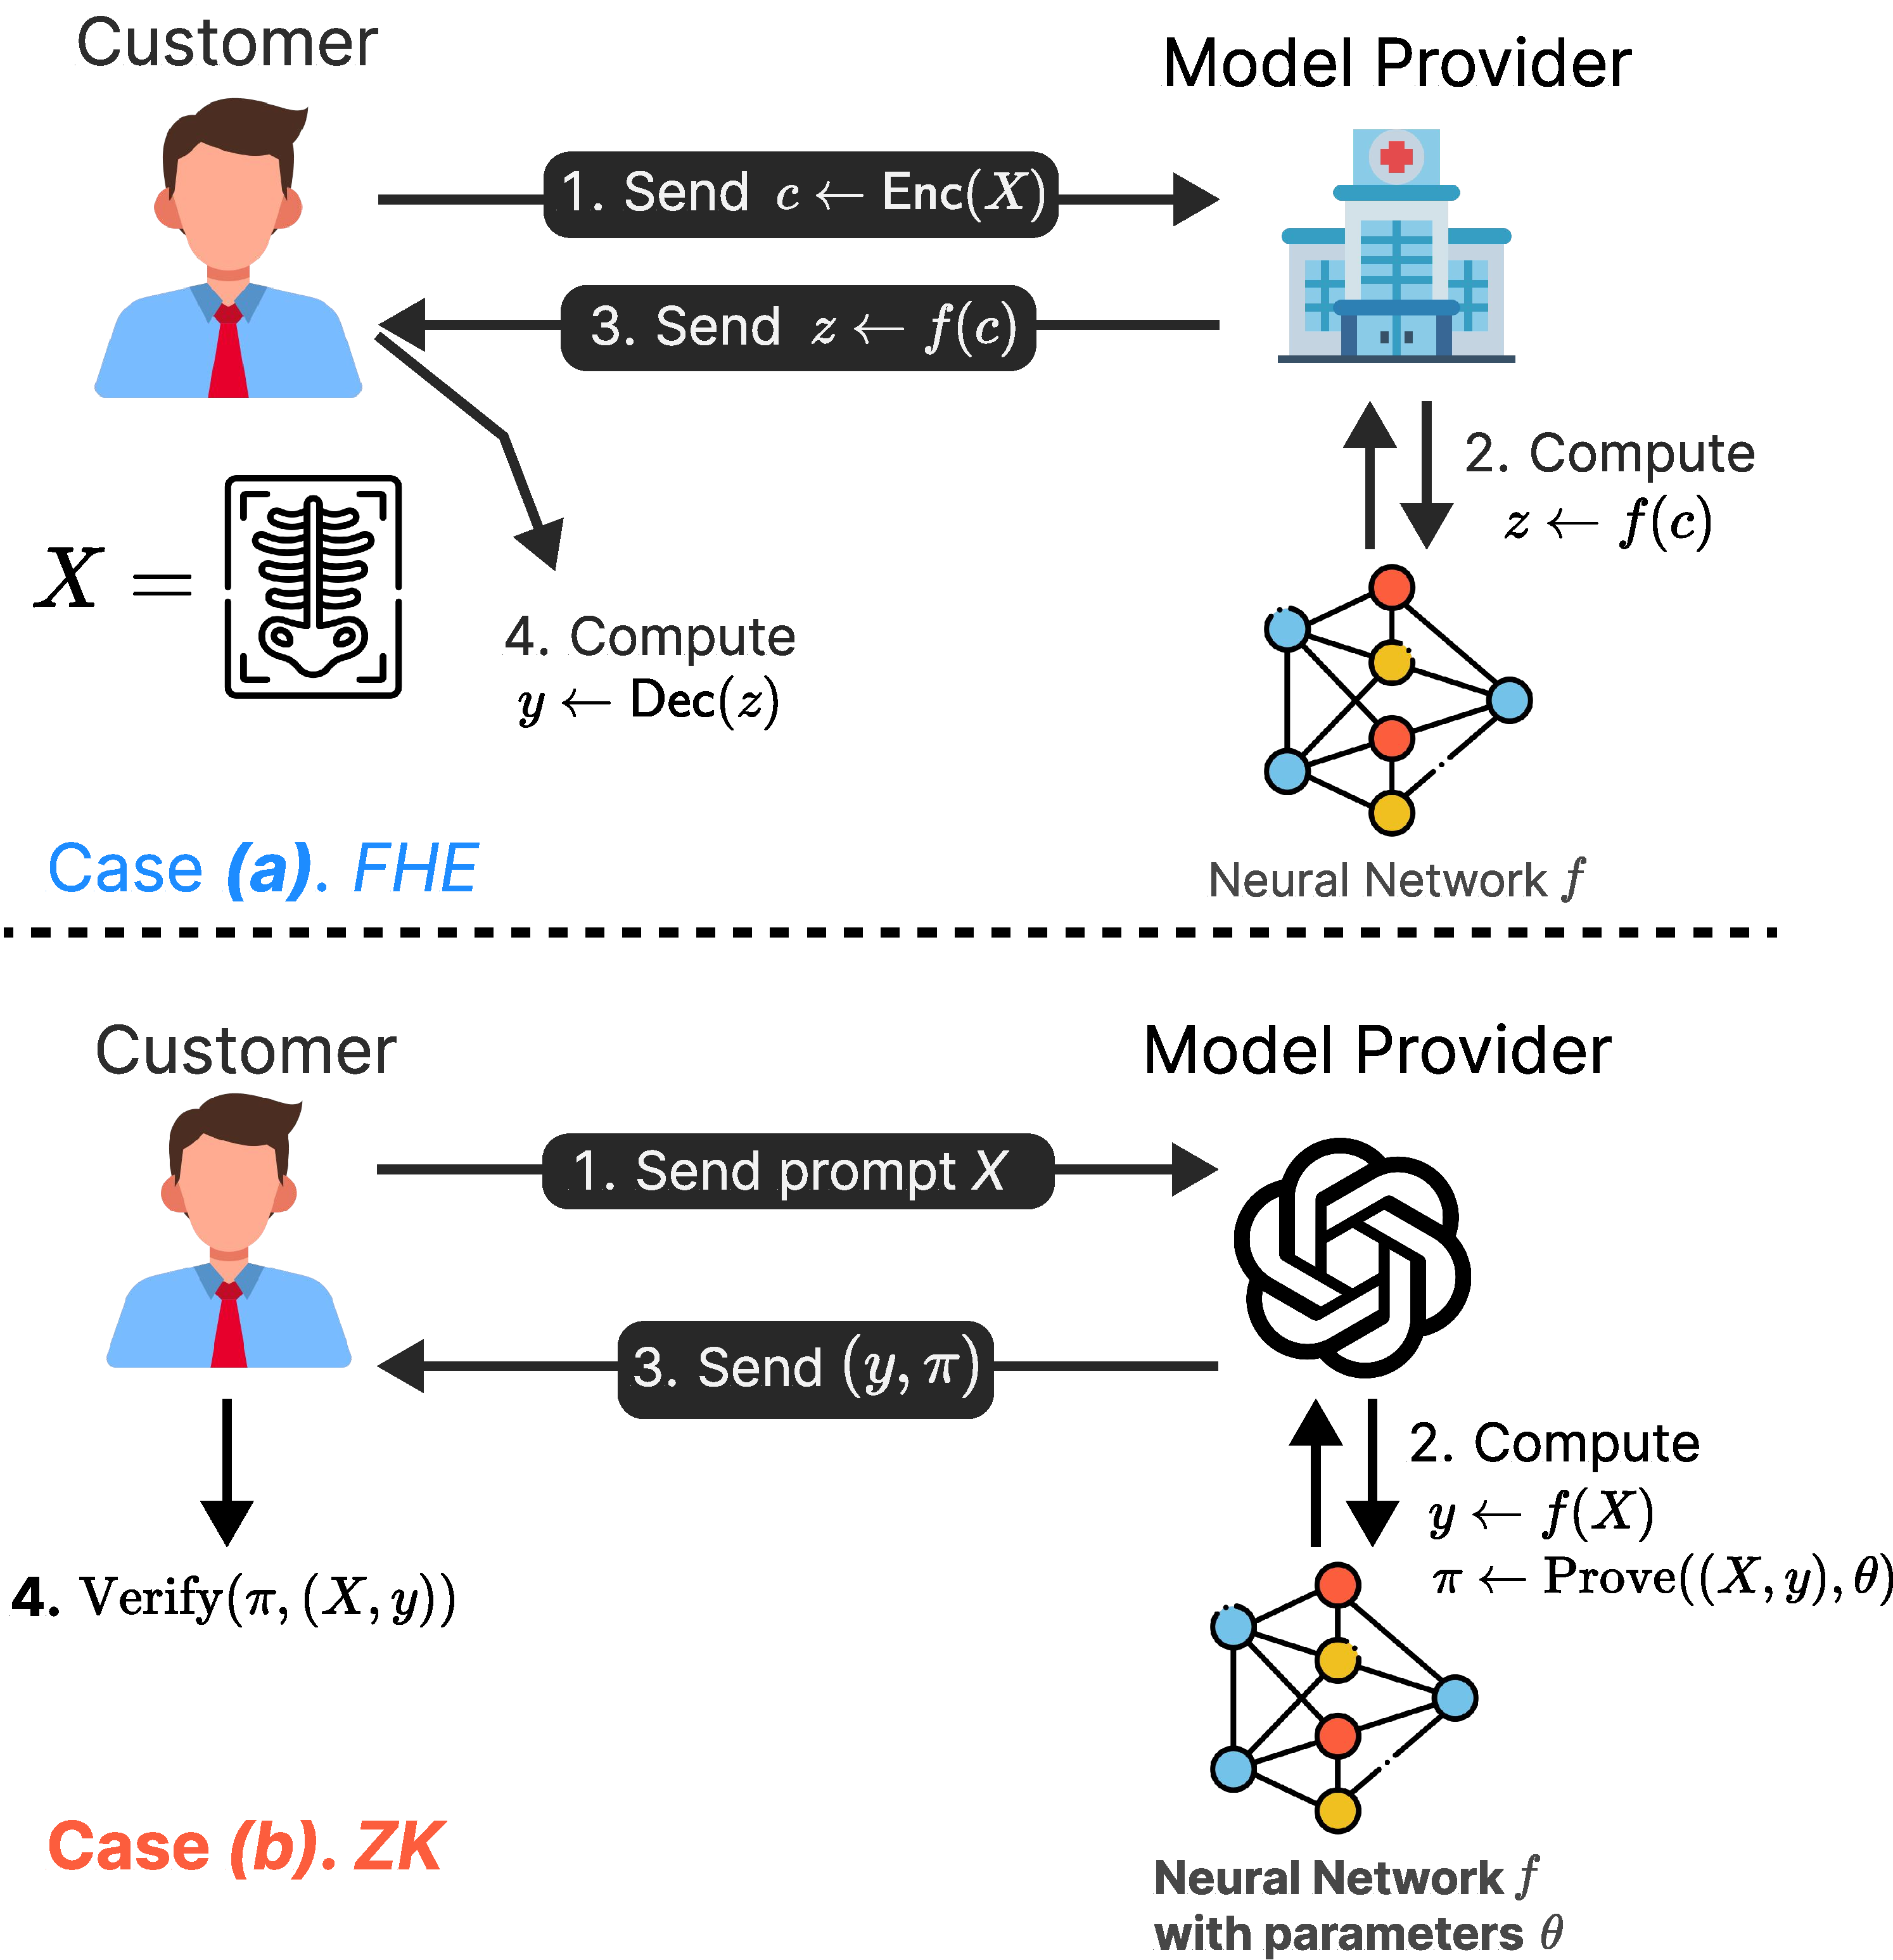
\includegraphics[width=0.8\textwidth]{figures/use-cases.pdf}
    \caption{Privacy concerns in neural networks. \textcolor{blue}{\textbf{Case (a)}} shows 
    the privacy concern of sending the data $x$ to the neural network $f$ without
    revealing the data itself. The user encrypts the data $x$, sends to the 
    neural network $f$, and receives the encrypted output, which can be 
    decrypted by the user's key. \textcolor{red}{\textbf{Case (b)}} shows the use-case 
    of zero-knowledge proofs for proving the neural network inference. The user
    sends the public input $x$ to the private neural network $f$, and then
    gets the output $y$ with a proof $\pi$ that $y = f(x)$.}
    \label{fig:nn-privacy}
\end{figure}

However, with the rise of neural networks, the rise of privacy concerns has
followed. In particular, the following issues are of concern:
\begin{itemize}
    \item How can we send the data $x$ to the neural network $f$ without
    revealing the data $x$ itself? For example, can the person, having the
    medical image $x$, send it to the analyzing neural network $f$ for the
    diagnosis without revealing $x$ \cite{cryptonets}? This example is illustrated 
    in \Cref{fig:nn-privacy}, case \textbf{(a)}.
    \item How can we trust the output of the neural network? In other words,
    given input $x$ and output $y$ of the neural network $f$, how can we be sure
    that $y = f(x)$ \cite{nn-ezkl}? This example is similarly illustrated in
    \Cref{fig:nn-privacy}, case \textbf{(b)}.
    \item How can we prove that the neural network $f$ was trained on the 
    non-sensitive data \cite{zk-training}? Can we train the neural network $f$ on the encrypted
    dataset \cite{fhe-training}?
\end{itemize}

To address these issues, the fields of zero-knowledge proofs (ZKP) and fully
homomorphic encryption (FHE) have been actively researched to work on top of
neural networks, which we introduce in the \Cref{section:preliminaries}. Despite
the progress in the field, the biggest bottleneck is the activation functions
used in neural networks. The activation functions are the non-linear
transformations applied to the intermediate outputs of the neural network and
are the core reason why the neural networks can approximate complex behaviours.
Despite this, the activation functions complicate the arithmetization of the
neural network inference for ZKP and FHE systems. We outline the core reasons 
in the \Cref{section:preliminaries}.

\subsection{Our Contribution}\label{section:our_contribution}

In this paper, we introduce the concept of \textit{activation-efficient neural
network architectures}. We analyze whether the activation functions used in
neural networks can be optimized for the sake of making them more
``cryptographically friendly''. We propose a novel approach to designing neural
network architectures that are more compatible with the existing
arithmetizations of cryptographic primitives. We show that the proposed
activation-efficient neural network architectures can be used to improve the
efficiency of zero-knowledge proofs and fully homomorphic encryption systems
working on top of neural networks.

\section{Applications}\label{section:preliminaries}

\subsection{Neural Networks}

The neural network, vaguely speaking, is the complicated parameterized function 
$f(x;\theta)$, taking a high-dimensional input $x$
and outputting the \textit{prediction result} $y$ using \textit{weights} $\theta$. 

The most basic task in training neural networks is the so-called
\textit{supervised learning}. Suppose we are given the supervised dataset
$\mathcal{D} = \{(\mathbf{x}_i, \mathbf{y}_i)\}_{i \in [N]}$ and we want to
train the neural network $f$ to have $f(\mathbf{x}_i) \approx \mathbf{y}_i$ (for
example, $\mathbf{x}_i$ might be an image of either cat or dog while $y_i \in
\{0,1\}$ is the image's label). We encapsulate our metric of model's ``badness''
in the loss function $\mathcal{L}$. For example, we might want to minimize the 
mean-squared error (MSE) on the given dataset:
\begin{equation*}
    \mathcal{L}(\mathcal{D};\theta) = \frac{1}{N} \sum_{i \in [N]} \left\|f(\mathbf{x}_i;\theta) - \mathbf{y}_i\right\|_2^2
\end{equation*}

Evidently, $\mathcal{L}$ is a function of parameters $\theta$ and the goal of the training
process is to find the optimal $\theta^* =
\arg\min_{\theta}\mathcal{L}(\mathcal{D};\theta)$ that minimizes the loss function. This
is typically done by the iterative methods such as Adam \cite{adam} or SGD
\cite{sgd}. So the typical optimization flow on the $j^{\text{th}}$ step, if 
SGD optimizer is used, might be:
\begin{equation*}
    v_j \gets \mu v_{j-1} + \eta \nabla_{\theta}\mathcal{L}(\mathcal{D};\theta), \quad \theta \gets \theta - v_j,
\end{equation*}

where $\eta \ll 1$ is the learning rate and $\mu$ is the momentum (typically
chosen between $0.9$ and $1.0$).

\subsection{Zero-Knowledge Proofs}

Suppose we have a statement $\mathbbm{x}$ with the corresponding witness
$\mathbbm{w}$ (we typically write $(\mathbbm{x}, \mathbbm{w}) \in \mathcal{R}$
for some relation $\mathcal{R}$). Typically, witness is some secret data that
proves the statement $\mathbbm{x}$ is true in polynomial or sub-polynomial time.
For example, the statement $\mathbbm{x}$ can be ``I know the discrete logarithm
of element $h := g^{\alpha}$ in the cyclic group $\mathbb{G} = \langle g
\rangle$ of order $q$'', and thus the witness $\mathbbm{w}$ can be the value of
$\alpha \in \mathbb{Z}_q$ while $\mathbbm{x} = h \in \mathbb{G}$. The
zero-knowledge proof systems have been extensively used in various applications,
ranging from blockchain scalability solutions to privacy-preserving identity
protocols \cite{snark-survey}.

There are numerous types of zero-knowledge proof systems nowadays:
$\Sigma$-proofs, zk-SNARKs \cite{snark-stark-comparison}, zk-STARKs
\cite{stark}, Bulletproofs \cite{bulletproofs} etc, each balancing 
the trade-offs between the proof size, verification time, and proving time.

However, the majority of widely used zero-knowledge proofs are the so-called
zk-SNARKs (zero-knowledge succinct non-interactive argument of knowledge). Let
us briefly describe the zk-SNARKs.

\begin{definition}
    A zk-SNARK is a zero-knowledge proof system protocol that allows one to
    prove the knowledge of a witness $\mathbbm{w}$ for a statement $\mathbbm{x}$
    for relation $\mathcal{R}$ in zero-knowledge. The zk-SNARK consists of the
    following algorithms:
    \begin{itemize}
        \item $\mathrm{KeyGen}(1^{\lambda}) \to (\mathsf{pp},\mathsf{vp})$: the
        key generation algorithm that generates the proving parameters
        $\mathsf{pp}$ and the verification parameters $\mathsf{vp}$ based on
        security parameter $\lambda \in \mathbb{N}$.
        \item $\mathrm{Prove}(\mathsf{pp}, \mathbbm{x}, \mathbbm{w}) \to \pi$: the
        proving algorithm that generates the proof $\pi$ for the statement
        $\mathbbm{x}$ with the witness $\mathbbm{w}$, based on the proving 
        parameters $\mathsf{pp}$.
        \item $\mathrm{Verify}(\mathsf{vp}, \pi, \mathbbm{x}) \to \{0, 1\}$: the
        verification algorithm that checks whether the proof $\pi$ is valid for
        the statement $\mathbbm{x}$ and outputs the bit $1$ if the proof is
        valid and $0$ otherwise.
    \end{itemize}

    Moreover, zk-SNARK satisfies the following properties:
    \begin{itemize}
        \item \textbf{Completeness:} for every statement $\mathbbm{x}$ and the
        corresponding witness $\mathbbm{w}$ (such that $(\mathbbm{x},
        \mathbbm{w}) \in \mathcal{R}$), the proof $\pi$ generated by the proving
        algorithm is valid:
        \begin{equation*}
            \text{Pr}\left[ \mathrm{Verify}(\mathsf{vp}, \pi, \mathbbm{x})=1 \;\middle|\; 
            \begin{matrix}
                (\mathsf{pp}, \mathsf{vp}) \gets \mathrm{KeyGen}(1^{\lambda}) \\
                \pi \gets \mathrm{Prove}(\mathsf{pp}, \mathbbm{x}, \mathbbm{w}) \\
                (\mathbbm{x}, \mathbbm{w}) \in \mathcal{R}
            \end{matrix}
            \right] = 1
        \end{equation*}
        \item \textbf{Soundness:} for every statement $\mathbbm{x}$ and the
        corresponding witness $\mathbbm{w}$ (such that $(\mathbbm{x},
        \mathbbm{w}) \notin \mathcal{R}$), the proof $\pi$ generated by the
        proving algorithm is invalid with overwhelming probability. Formally, 
        for all PPT adversaries $\mathcal{A}$:
        \begin{equation*}
            \text{Pr}\left[ \mathrm{Verify}(\mathsf{vp}, \pi, \mathbbm{x})=1 \;\middle|\; 
            \begin{matrix}
                (\mathsf{pp}, \mathsf{vp}) \gets \mathrm{KeyGen}(1^{\lambda}) \\
                (\mathbbm{x}, \mathbbm{w}) \gets \mathcal{A}(\mathsf{pp}, \mathsf{vp}) \\
                \pi \gets \mathrm{Prove}(\mathsf{pp}, \mathbbm{x}, \mathbbm{w})
            \end{matrix}
            \right] = \mu(\lambda),
        \end{equation*}
        where $\mu$ is negligible in $\lambda$, that is $\lim_{\lambda \to
        \infty}\mu(\lambda)\lambda^{\gamma}=0$ for all $\gamma \in \mathbb{R}$.
        \item \textbf{Argument of Knowledge:} for every statement $\mathbbm{x}$,
        the proof $\pi$ ensures the verifier that the prover \textit{knows} the
        witness $\mathbbm{w}$ for the statement $\mathbbm{x}$.
        \item \textbf{Zero-Knowledge:} for every statement $\mathbbm{x}$ and the
        corresponding witness $\mathbbm{w}$, the proof $\pi$ does not reveal any information about the witness
        $\mathbbm{w}$.
        \item \textbf{Succinctness:} the proof $\pi$ generated by the proving
        algorithm is of polylogarithmic size in the size of the computatinal
        problem $N$ as well as the verification time $T$. In other words,
        typically we have $|\pi| = \mathcal{O}_{\lambda}(\log^{\alpha} N)$ and
        $T=\mathcal{O}_{\lambda}(\log^{\beta} N,|\mathbbm{x}|)$.
    \end{itemize}
\end{definition}

For more information on zk-SNARKs, we refer the reader to \cite{zksnark}.

However, to properly use zero-knowledge systems, one needs to somehow
arithmetize the relation $\mathcal{R}$. Arithmetization always involves working
over some finite field $\mathbb{F}$ (for concreteness, one might think of the
prime field $\mathbb{F} = \mathbb{F}_p$ for some prime $p$). One of two most
common ways to arithmetize the relations is to either use R1CS (Rank-1
Constraint Systems) or $\mathcal{P}$lon$\mathcal{K}$ish arithmetization.
Regardless of the choice, the primary challenge of verifying whether $y=f(x)$
are the following:
\begin{itemize}
    \item All operations must be conducted over the field $\mathbb{F}$.
    \item Each multiplication and addition operation adds a new constraint to
    the system, increasing dramatically the proving time and the proof size in
    certain proving systems. For example, as benchmarked in \cite{spartan}, the
    proving time of $2^{20} \approx 10^6$ constraints can take more than a
    minute in the Groth16 proving system \cite{groth16}, roughly two minutes in
    Ligero \cite{ligero}, and up to eight minutes in Hyrax \cite{hyrax}.
    \item Only addition and multiplication operations over two inputs are
    allowed.
\end{itemize}

Such arithmetization of $f$ is called the \textbf{arithmetical
circuit}\footnote{Formally, arithmetical circuit $C: \mathbb{F}^n \to
\mathbb{F}^m$ is a directed acyclic graph with nodes labeled with $+$, $-$, or
$\times$. Essentially, any arithmetical circuit defines an $n$-variate
polynomial with an evaluation recipe.}, which we denote by $C_f$. Further, by
$\mathsf{A}$ we cost of addition, by $\mathsf{M}$ we denote the cost of the
multiplication operation. Finally, we specify the following theorem to
understand the prover's complexity in terms of the number of additions and
multiplications.

\begin{theorem}
    Let $C_f$ be the arithmetical circuit of $f$. Let $a$ be the number of
    additions and $m$ be the number of multiplications, used in $C_f$: that is,
    the total cost of circuit evaluation is $a\mathsf{A} + m\mathsf{M}$. Then,
    the most common prover's time complexity in R1CS is
    $\mathcal{O}_{\lambda}(m\log m)$, while in $\mathcal{P}$lon$\mathcal{K}$ish
    arithmetization it is $\mathcal{O}_{\lambda}((m+a)\log(m+a))$.
\end{theorem}

% \begin{definition}[R1CS Arithmetization \cite{groth16}]
%     Fix the finite field $\mathbb{F}$. R1CS arithmetization consists of three
%     matrices $L$, $R$, and $O \in \mathbb{F}^{m \times n}$ which, given 
%     the public statement $\mathbbm{x} \in \mathbb{F}^{\ell}$ and the 
%     witness $\mathbbm{w} \in \mathbb{F}^{n-\ell-1}$, satisfy the following
%     relation:
%     \begin{equation*}
%         \mathcal{R}_{\text{R1CS}} = \left\{ 
%             (\mathbbm{x}, \mathbbm{w}) \in \mathbb{F}^{\ell} \times \mathbb{F}^{n-\ell-1} \; \middle| \; 
%             \begin{matrix}
%                 \mathbf{z} = (\mathbbm{w}, \mathbbm{x}, 1) \in \mathbb{F}^n \\
%                 L\mathbf{z} \odot R\mathbf{z} = O\mathbf{z}
%             \end{matrix}
%         \right\}
%     \end{equation*}

%     The number $n$ is called the \textbf{witness size}, while the number $m$ is called the
%     \textbf{number of constraints}.
% \end{definition}

% \begin{definition}[$\mathcal{P}$lon$\mathcal{K}$ish Arithmetization \cite{plonk}]
%     The $\mathcal{P}$lon$\mathcal{K}$ish arithmetization consists of left,
%     right, output selectors $\mathbf{q}_L, \mathbf{q}_R, \mathbf{q}_O \in
%     \mathbb{F}^{n}$, adding the left, right, and output wires
%     $(\boldsymbol{\ell}, \mathbf{r}, \mathbf{o}) \in \mathbb{F}^{3n}$, and
%     $\mathbf{q}_M$, multiplying left and right wires, and $\mathbf{q}_C$, adding
%     a public constant. This way, the relation $\mathcal{R}_{\text{PlonK}}$ is
%     defined as follows:
%     \begin{equation*}
%         \mathcal{R}_{\text{PlonK}} = \left\{ 
%             (\mathbbm{x}, \mathbbm{w}) \in \mathbb{F}^{\ell} \times \mathbb{F}^{n-\ell} \; \middle| \; 
%             \begin{matrix}
%                 \mathbf{z} = (\mathbbm{w}, \mathbbm{x}) \in \mathbb{F}^n \\
%                 \mathbf{q}_L \odot \boldsymbol{\ell} + \mathbf{q}_R \odot \mathbf{r} + \mathbf{q}_O \odot \mathbf{o} + \mathbf{q}_M \odot (\boldsymbol{\ell} \odot \mathbf{r}) + \mathbf{q}_C = \mathbf{0}
%             \end{matrix}
%         \right\}
%     \end{equation*}

%     The number $n$ is called the \textbf{number of gates}.
% \end{definition}

% Let us consider how to arithmetize certain operations to better understand the
% challenges of arithmetization.

% \begin{example}
%     Suppose the program consists in verifying whether $y=x^4+x^2+1$. To write down
%     the relations $\mathcal{R}_{\text{R1CS}}$ and $\mathcal{R}_{\text{PlonK}}$,
%     we need to write down the calculation of $y$ as the system of quadratic
%     equations. More specifically,
%     \begin{align*}
%         t_1 &= x^2, \\
%         t_2 &= x \cdot t_1, \\
%         t_3 &= x \cdot t_2, \\
%         y &= t_3 + t_1 + 1
%     \end{align*}
% \end{example}

\subsection{Homomorphic Encryption}

One of the use-cases of activation efficient neural networks is the usage of the
so-called \textit{homomorphic encryption} (HE) schemes. Roughly speaking, such
schemes allows one to encrypt two plaintexts (say, $m_1$ and $m_2$), encrypt
them: $c_1 \gets \mathsf{Enc}(m_1), c_2 \gets \mathsf{Enc}(m_2)$, and then
perform some operations on the ciphertexts (typically, additions and
multiplications), which will result in the encryption $c=f(c_1,c_2)$ that, after
decryption, will be equal to the result of the operation performed on the
plaintexts: $f(m_1,m_2) = \mathsf{Dec}(c)$. Similarly to the zero-knowledge
proofs, the homomorphic encryption schemes support only addition and 
multiplication operations over the certain finite structure.

Now, let us properly define the homomorphic encryption scheme.
\begin{definition}[FHE Scheme]
    Fully Homomorphic Encryption (FHE) scheme is a tuple of algorithms
    $(\mathsf{KeyGen}, \mathsf{Enc}, \mathsf{Dec}, \mathsf{Eval})$:
    \begin{itemize}
        \item $\mathrm{KeyGen}(1^{\lambda}) \to (\mathsf{sk},\mathsf{ek})$: Given the 
        security parameter $\lambda \in \mathbb{N}$, outputs the secret key $\mathsf{sk}$
        kept secret by the user and public evaluation key $\mathsf{ek}$.
        \item $\mathrm{Enc}(\mathsf{sk},\mu) \to c$: Given the secret key $\mathsf{sk}$
        and message $\mu$, outputs the ciphertext $c$.
        \item $\mathrm{Dec}(\mathsf{sk},c) \to \mu$: Given the secret key
        $\mathsf{sk}$ and ciphertext $c$, outputs the message $\mu$.
        \item $\mathrm{Eval}(\mathsf{ek},f,c_1,\ldots,c_{\ell}) \to
        \widetilde{c}$: Given the evaluation key $\mathsf{ek}$, function $f \in
        \mathcal{F}$ from the supported class of functions $\mathcal{F}
        \subseteq \{f: \mathbb{Z}^{\ell}_2 \to \mathbb{F}\}$, and ciphertexts
        $c_1,\ldots,c_{\ell}$, outputs the ciphertext of the result of the
        function $f$ applied to the plaintexts corresponding to the ciphertexts.
    \end{itemize}
    We require the following properties:
    \begin{itemize}
        \item \textbf{Correctness:} for every supported circuit $f \in \mathcal{F}$ and 
        inputs $\mu_1,\dots,\mu_{\ell}$, we have
        \begin{equation*}
            \text{Pr}\left[ \mathsf{Dec}(\mathsf{sk},\widetilde{c}) = f(\mu_1,\dots,\mu_{\ell}) \; \middle| \; \begin{matrix}
                (\mathsf{sk},\mathsf{ek}) \gets \mathsf{KeyGen}(1^{\lambda}) \\
                c_j \gets \mathsf{Enc}(\mathsf{sk},\mu_j), j \in [\ell], \\
                \widetilde{c} \gets \mathsf{Eval}(\mathsf{ek},f,c_1,\dots,c_{\ell})
            \end{matrix} \right] \geq 1 - \mu(\lambda)
        \end{equation*}
        \item \textbf{Semantic Security:} for any two messages $\mu_0,\mu_1$
        it holds that
        \begin{equation*}
            \left\{ (\mathsf{ek},c_0): \begin{matrix}
                (\mathsf{sk},\mathsf{ek}) \gets \mathsf{KeyGen}(1^{\lambda}) \\
                c_0 \gets \mathsf{Enc}(\mathsf{sk},\mu_0)
            \end{matrix} \right\} \approx_C \left\{ (\mathsf{ek},c_1): \begin{matrix}
                (\mathsf{sk},\mathsf{ek}) \gets \mathsf{KeyGen}(1^{\lambda}) \\
                c_0 \gets \mathsf{Enc}(\mathsf{sk},\mu_1)
            \end{matrix} \right\},
        \end{equation*}
        where $\approx_C$ means the computational indistinguishability.
        \item \textbf{Compactness:} for every circuit $f \in \mathcal{F}$ and
        inputs $\mu_1,\dots,\mu_{\ell}$, let 
        \begin{align*}
        &(\mathsf{sk},\mathsf{ek}) \gets
        \mathsf{KeyGen}(1^{\lambda}), \\
        &c_j \gets \mathsf{Enc}(\mathsf{sk},\mu_j), \; j \in [\ell], \\
        &\widetilde{c} \gets \mathsf{Eval}(\mathsf{ek},f,c_1,\dots,c_{\ell})
        \end{align*}
        Then, sizes $\{|c_j|\}_{j \in [\ell]}$ and $|\widetilde{c}|$ depend only
        on the security parameter $\lambda$ and independent of both the size
        $|f|$ and $\ell$.
    \end{itemize}
\end{definition}

Now, let us consider the concrete fully homomorphic encryption scheme, namely
the GSW scheme, introduced in \cite{gsw}. At a high level, the GSW utilizes the
idea that the eigenvectors of matrices are preserved under the matrix addition
and multiplication. Indeed, if $\mathbf{v}$ is the eigenvector of both $C_1$ and
$C_2$ with eigenvalues $\lambda_1$ and $\lambda_2$, respectively, then
$C_1\mathbf{v}=\lambda_1\mathbf{v}$, $C_2\mathbf{v}=\lambda_2\mathbf{v}$, and
$(C_1+C_2)\mathbf{v}=(\lambda_1+\lambda_2)\mathbf{v}$, as well as
$(C_1C_2)\mathbf{v}=\lambda_1\lambda_2\mathbf{v}$. That is, $\mathbf{v}$ is the
eigenvector of $C_1+C_2$ and $C_1C_2$ with eigenvalues $\lambda_1+\lambda_2$ and
$\lambda_1\lambda_2$, respectively. That being said, we will use eigenvector as
the secret key, matrices as the ciphertexts, while the corresponding eigenvalues
are the messages to be encrypted. Unfortunately, this way such scheme would not
be secure as finding the eigenvectors is computationally easy. Therefore, we
introduce the noise (error) term $\mathbf{e}$, changing the ciphertext/secret
key relation to $C\mathbf{s}=\mu\mathbf{v}+\mathbf{e}$, where $\mu \in
\mathbb{Z}_2$ is a message. Let us now give the formal definition of the GSW
scheme.

\begin{definition}[GSW Scheme.]
    Fix parameters $(m,n,q,\chi)$ with sufficiently large $m$ and some
    distribution $\chi$. Let $\ell := (n+1)\log q$. Construction then works as
    follows:
    \begin{itemize}
        \item $\mathrm{KeyGen}(1^{\lambda}) \to \mathbf{s} \in
        \mathbb{Z}_q^{n+1}$. Sample a random vector $\mathbf{s}' \xleftarrow{R}
        \mathbb{Z}_q^n$ and output the vector $\mathbf{s} = (-\mathbf{s}',1) \in
        \mathbb{Z}_q^{n+1}$ as the secret key.
        \item $\mathrm{Enc}(\mathbf{s} \in \mathbb{Z}_q^{n+1},\mu \in
        \mathbb{Z}_2) \to C \in \mathbb{Z}_q^{\ell \times (n+1)}$. Sample the 
        random matrix $A \xleftarrow{R} \mathbb{Z}_q^{\ell \times n}$ and 
        error vector $\mathbf{e} \xleftarrow{R} \chi^{\ell}$. Build the 
        matrix $B = (A,A\mathbf{s}'+\mathbf{e}) \in \mathbb{Z}_q^{\ell \times (n+1)}$
        and output $C = B + \mu G$ for some fixed matrix $G$.
        \item $\mathrm{Dec}(\mathbf{s} \in \mathbb{Z}_q^{n+1},C \in
        \mathbb{Z}_q^{\ell \times (n+1)}) \to \mu \in \mathbb{Z}_2$. Compute the
        vector $\mathbf{v} = C\mathbf{s}$. Output $0$ if
        $\|\mathbf{v}\|_{\infty}<\delta q$ for small $\delta$ (that is,
        $\|\mathbf{v}\|_{\infty}$ is small, e.g., $\delta \approx \frac{1}{4}$),
        otherwise output $1$.
    \end{itemize}
\end{definition}

\textbf{Correctness.} Let us check why such scheme is correct. Take the message $\mu \in \mathbb{Z}_2$
and encrypt it:
\begin{equation*}
    C \gets \mathsf{Enc}(\mathbf{s},\mu) = (A,A\mathbf{s}'+\mathbf{e}) + \mu G
\end{equation*}

Based on the LWE (Learning With Errors) assumption (more on that can be found in
\cite{lwe}), we have that $(A,A\mathbf{s}'+\mathbf{e}) \approx_C (A,\mathbf{u})$
for some random $A$ and random $\mathbf{u} \in \mathbb{Z}_q^m$. Therefore, the
expression $(A,A\mathbf{s}'+\mathbf{e}) + \mu G$ is indistinguishable from
random, thus the scheme is secure. Now, suppose we know the secret $\mathsf{s}$
and multiply it by the ciphertext:
\begin{equation*}
    \mathbf{v} = C\mathbf{s} = (A,A\mathbf{s}'+\mathbf{e})\begin{pmatrix}
        -\mathbf{s}' \\ 1
    \end{pmatrix} + \mu G \begin{pmatrix}
        -\mathbf{s}' \\ 1
    \end{pmatrix} = \mu G \mathbf{s} + \mathbf{e}
\end{equation*}

If $\mu=0$, then $\mathbf{v} = \mathbf{e}$, which is small. If $\mu=1$, then
$\mathbf{v} = \mathbf{e} + G\mathbf{s}$ and since $\mathbf{s}$ is arbitrary and
$G$ is fixed, the expression $G\mathbf{s}$ is indistinguishable from random,
thus $\|\mathbf{v}\|_{\infty}$ should have a large norm (close to
$\frac{1}{2}q \gg \delta q$).

\textbf{Homomorphic Operations.} To add two ciphertexts $C_1$ and $C_2$, we
simply add them together: $C_1 \oplus C_2 \triangleq C_1 + C_2$. Indeed, if we are to 
decrypt the sum $C$, we would have:
\begin{equation*}
    C\mathbf{s} = C_1\mathbf{s} + C_2\mathbf{s} = (\mu_1 G\mathbf{s}+\mathbf{e}_1) + (\mu_2 G\mathbf{s} + \mathbf{e}_2)
    = \textcolor{blue}{\underbrace{(\mu_1+\mu_2)}_{\text{new message}}}G\mathbf{s} + \textcolor{red}{\underbrace{(\mathbf{e}_1+\mathbf{e}_2)}_{\text{new error}}}
\end{equation*}

To define the product, we need an auxiliary function $\phi: \mathbb{Z}_q^{\ell
\times (n+1)} \to \mathbb{Z}_q^{\ell \times (n+1)\log q}$ such that entries of 
$\phi(C)$ are all small (namely, they are in $\mathbb{Z}_2$) and the function 
$\phi$ is the inverse to the matrix $G$, that is $\phi(C)G=C$. 

In this case, the product of two ciphertexts $C_1$ and $C_2$ is defined as $C_1
\otimes C_2 \triangleq \phi(C_1)C_2$. Decryption in such case is conducted as follows:
\begin{align*}
    (C_1 \otimes C_2)\mathbf{s} = \phi(C_1)(\mu_2 G\mathbf{s} + \mathbf{e}_2) &= \mu_2 \phi(C_1)G\mathbf{s} + \phi(C_1)\mathbf{e}_2 \\
    &= \mu_2C_1 \mathbf{s} + \phi(C_1)\mathbf{e}_2 \\
    &= \mu_2(\mu_1 G\mathbf{s} + \mathbf{e}_1) + \phi(C_1)\mathbf{e}_2\\
    &= \textcolor{blue}{\underbrace{(\mu_1\mu_2)}_{\text{new message}}}G\mathbf{s} + 
    \textcolor{red}{\underbrace{(\mu_2\mathbf{e}_1 + \phi(C_1)\mathbf{e}_2)}_{\text{new error}}}
\end{align*}

\textbf{Error Propagation.} The error propagation in the GSW scheme is the
primary bottleneck which limits the number of operations that can be performed
over the ciphertexts. To see why, consider the following proposition.

\begin{proposition}
    After each addition, the error in the GSW scheme is roughly doubled, while
    after each multiplication the error is multiplied by roughly $n\log q$. 
\end{proposition}

For that reason, we are oftentimes limited not only in terms of the execution
time, but also in terms of the error that accumulates after each operation. For
that reason, it is essential to reduce the error in the ciphertexts, which can
be achieved partially by utilizing the activation-efficient neural networks.

\section{Activation-Efficient Neural Networks}

\subsection{Arithmetical Circuits for Neural Networks}

Now, the main question arises: can we theoretically design the arithmetical 
circuit (both for zero-knowledge proofs and homomorphic encryption) in such a
way that it represents the neural network prediction with the appropriate 
accuracy? The answer is yes, which was specified in \cite{cryptonets}. 
The primary theorem is the following.

\begin{theorem}
    Let $f$ be a neural network with continuous non-linear transformations. Let
    $X \subset \mathbb{R}^n$ be compact. Then, for every $\varepsilon > 0$ there 
    exists a polynomial $p$ such that:
    \begin{equation*}
        \sup_{\mathbf{x} \in X}\|f(\mathbf{x}) - p(\mathbf{x})\| < \varepsilon
    \end{equation*}
\end{theorem}

In other words, the neural network can be approximated by a polynomial with the
arbitrary accuracy. Since any polynomial can be encoded as the arithmetical
circuit, we can design the arithmetical circuit that represents the neural
network prediction with the arbitrary accuracy. For that reason, we 
provide the following theorem, following the original study \cite{cryptonets}.

\begin{theorem}
    Let $(\mathsf{Enc}, \mathsf{Dec})$ be the encryption and decryption
    functions of a FHE system. Let $f: \mathbb{R}^n \to \mathbb{R}^m$ be the
    neural network consisting of continuous non-linear transformations. Let $X
    \subset \mathbb{R}^n$ be a compact. Suppose $\mathsf{sk}$ be the properly
    generated secret key. Then, for every $\varepsilon > 0$ there exists a
    circuit $\widetilde{f}$ such that
    \begin{equation*}
        \sup_{\mathbf{x} \in X}\|f(\mathbf{x}) - \mathsf{Dec}(\mathsf{sk}, \widetilde{f}(\mathsf{Enc}(\mathsf{sk},\mathbf{x})))\| < \varepsilon
    \end{equation*}
\end{theorem}

Finally, we provide the theorem that connects the zero-knowledge proofs and
the approximation of the neural networks.

\begin{theorem}
    Suppose $f(\star; \boldsymbol{\theta}): \mathbb{R}^n \to \mathbb{R}^m$ is
    the neural network, parameterized by weights $\boldsymbol{\theta}$. The
    prover, provided with the public input $\mathbf{x}$, wants to prove that
    $\mathbf{y} = f(\mathbf{x}; \boldsymbol{\theta})$ holds without revealing
    the parameters $\boldsymbol{\theta}$. Suppose $\mathsf{Enc}: \mathbb{R}^n
    \to \mathbb{F}^n$ encodes the real-valued vector to the vector of field
    elements while $\mathsf{Dec}: \mathbb{F}^m \to \mathbb{R}^m$ decodes it
    back. Then, for every $\varepsilon > 0$ there exists an arithmetical circuit
    $C_f$ such that the proving system over the relation
    \begin{equation*}
        \mathcal{R} = \left\{ \begin{matrix}
            \mathbbm{x} = (\mathbf{x}, \mathbf{y}, \varepsilon) \in \mathbb{R}^{n} \times \mathbb{R}^m \times \mathbb{R}_{> 0} \\
            \mathbbm{w} = (\boldsymbol{\theta})
        \end{matrix} \; \middle| \; \begin{matrix}
            \sup_{\mathbf{x} \in X}\left\|f(\mathbf{x}; \boldsymbol{\theta}) - \mathsf{Dec} \circ C_f \circ \mathsf{Enc}(\mathbf{x})\right\| < \varepsilon
        \end{matrix} \right\}
    \end{equation*}
    is complete and sound over the compact $X \subset \mathbb{R}^n$.
\end{theorem}

While the above two theorems provide the solid theoretical foundation, they do
not help to design the circuits specifically and do not provide the
computational efficiency of executing and using protocols over such circuits. Up
until this point, the majority of existing approaches produce the cryptographic
schemes that require the overwhelming resources to be used: see \cite{zkml}, for
instance. The biggest bottleneck is the large matrix multiplications and 
non-linearities that are computationally expensive. Among these two issues,
we try to mitigate the non-linearities by designing neural networks 
that use as few non-linearities as possible.

\subsection{Activations in Neural Networks}

Throughout the years, the neural network community has introduced a variety of
activation functions which are used for different purposes. In this section, we
provide the list of the most common activation functions and their compatibility
with zero-knowledge proofs, homomorphic encryption, and optimization. The list
is provided in \Cref{table:activations}.

\begin{table}[H]
    \centering
    \begin{tabular}{cccc}
        \hline
        \textbf{Name} & \textbf{Formula} & \textbf{Where used?} \\
        \hline
        ReLU & $\max\{0,x\}$ & Cost-effective non-linearity \\
        $\text{LeakyReLU}_{\alpha}$ & $\max\{\alpha x,x\}$ & Cost-effective non-linearity \\
        Sigmoid $\sigma(x)$ & $\frac{1}{1+e^{-x}}$ & Binary classification \\
        Tanh & $\frac{1-e^{-2x}}{1+e^{-2x}}$ & Binary classification \\
        Softmax & $\left\{e^{x_i}/\sum_{j\in [n]}e^{x_j}\right\}_{i \in [n]}$ & Multi-class classification \\
        Swish & $x\sigma(x)$ & General-purpose non-linearity \\
        \hline
    \end{tabular}
    \caption{The most common activation functions and their applications.}
    \label{table:activations}
\end{table}

Now, suppose given the activation function $g: \mathbb{R} \to \mathbb{R}$, 
our problem is to design the arithmetical circuit that represents the function
$g$. One of the widely used methods is to approximate the function $g$ by the
polynomial $\widetilde{g}$ of the degree $d$. For example, this can be done using 
the Taylor series expansion:
\begin{equation*}
    \widetilde{g}(x) = \sum_{k=0}^d c_k x^k + \mathcal{O}(x^{d+1}), \quad c_k = \frac{g^{(k)}(0)}{k!}
\end{equation*}

Expansions of some of the most common activation functions are provided in
\Cref{table:activations-appr}. For example, the ReLU function can be approximated by
the polynomial $0.47 + 0.5x + 0.09x^2$ or, if desirable, with even higher-order 
degrees. Then, to use the activation function in the arithmetical circuit, we
encode the coefficients $\{c_j\}_{j \in [d]}$ as the field elements and 
perform the polynomial evaluation over the field (or ring in FHE). 

However, the polynomial approximation proved itself to be inefficient due 
to the significant error induced during the whole neural network execution. 
This has a rigorous reasoning, included in \cite{not-polynomials}, which 
claims that every non-linear functions, \textbf{except for polynomials},
can approximate any continuous function on the compact. 

\begin{table}[H]
    \centering
    \begin{tabular}{cccc}
        \hline
        \textbf{Name} & \textbf{Approximation} \\
        \hline
        ReLU & $0.47 + 0.5x + 0.09x^2$ \\
        Tanh & $0.51x - 0.04x^3 + 0.0011x^5$ \\
        Swish & $0.24 + 0.5x + 0.1x^2$\\
        \hline
    \end{tabular}
    \caption{The most common activation functions and their applications.}
    \label{table:activations-appr}
\end{table}

This motivates us to use the activation functions that are not polynomials, yet
can be theoretically implemented in the arithmetical circuits. Obviously, all
candidates involving the exponential or trigonometric functions are not suitable
for the cryptographic protocols. For that reason, we consider the
$\mathsf{ReLU}$ function and its modifications as the target activation
functions. Our main claim is the following.
\begin{proposition}
    Implementing the $\mathsf{ReLU}$ function in the arithmetical circuit 
    requires roughly $\log_2 |\mathbb{F}|$ multiplication and $2\log_2 |\mathbb{F}|$ addition gates 
    where $\mathbb{F}$ is the underlying field.
\end{proposition}

\textbf{Proof.} The $\mathsf{ReLU}$ function is defined as $\mathsf{ReLU}(x) =
\max\{0,x\}$. To implement it in the arithmetical circuit, we need to check the
sign of $x$. For that reason, we need to decompose the number $x$ into the
binary representation: $x = \sum_{i=0}^{\ell-1}x_j2^j$ where $\ell =
\lceil\log_2 |\mathbb{F}|\rceil$. Since each $x_j$ must be either $0$ or $1$, we
impose the constraint $x_j(x_j-1) = 0$, costing us one multiplication and one
addition gate. Then, to sum all the $x_j$'s, we need additional
$\log_2|\mathbb{F}|$ addition gates. The total cost is thus
$\log_2|\mathbb{F}|\cdot\mathsf{M} + 2\log_2|\mathbb{F}|\cdot\mathsf{A}$.
Finally, if $x_s$ is the sign bit (for some fixed $s \in [\ell]$), it suffices to
output $x_s \cdot x$: if $x_s = 0$, then the output is $0$, otherwise the output
is $x$. This requires one additional multiplication gate. $\blacksquare$

This way, we can implement any ReLU-like functions in the arithmetical circuits
without losing the accuracy. Yet, what other functions are we left with?
MobileNet papers \cite{mobilenetv2,mobilenetv3} introduced the optimized
versions for sigmoid and swish functions, called \textit{hard sigmoid} and
\textit{hard swish}. To define them, consider the ReLU6 function:
\begin{equation*}
    \text{ReLU6}(x) = \min\{\max\{0,x\},6\}
\end{equation*}

Then, to define the hard sigmoid and hard swish functions, we use the following
formulas:
\begin{align*}
    \text{h-sigmoid}(x) &= \frac{1}{6}\text{ReLU6}(x-3) \\
    \text{h-swish}(x) &= x \cdot \text{h-sigmoid}(x)
\end{align*}

Note that such functions cost roughly twice as much as the ReLU function, since 
we need to perform two comparisons instead of one. However, they are still
efficient enough to be used in the cryptographic protocols.

Finally, the Softmax layer can be implemented as the regular maximum function:
instead of computing the vector $\textrm{Softmax}(\mathbf{x})$, we simply output
the one-hot vector $\mathbf{y}$ where $\mathbf{y}_i = \mathbf{1}[x_i =
\max_{j}x_j]$ with $\mathbf{1}[\cdot]$ being the indicator function.

\subsection{Optimizing the Number of Activations}

Another problem is the number of activations. Consider the simplest
construction: the neural network with the single layer. Dropping the bias term,
the forward pass is defined as $f(\mathbf{x}; W) = \sigma(W\mathbf{x})$ for
$\mathbf{x} \in \mathbb{R}^n$, $W \in \mathbb{R}^{m \times n}$, and $\sigma$ is
the activation function (think of ReLU). Now suppose we want to implement the
forward pass in the arithmetical circuit with the arbitrary field $\mathbb{F}$,
where its bitsize is $\ell := \lceil \log_2 |\mathbb{F}| \rceil$. What is the
complexity of such approach?

\begin{proposition}
    The complexity of the forward pass in the neural network with the single
    layer is $\mathcal{O}(m(n+\ell))$ multiplications and
    additions.
\end{proposition}

\textbf{Proof.} Note that the matrix-vector multiplication $W\mathbf{x}$ costs
$\mathcal{O}(mn)$ multiplications and additions. Then, the activation function
$\sigma$ costs $\mathcal{O}(\ell)$ multiplications and additions.
Since the activation function is applied to each element of the vector, the total
cost is $\mathcal{O}(m(n+\ell))$. $\blacksquare$

Is there any way to reduce the number of activations? The answer is yes. The 
core idea that we propose is to use the Encoder-Decoder architecture, where the
activation function is applied only to the output of the Encoder. Let us 
define the architecture.
\begin{definition}
    The \textbf{Encoder-Decoder layer} between $n$ and $m$ neurons in input and
    output, respectively, with $h$ hidden units, is defined as follows: let
    $E \in \mathbb{F}^{n \times h}$ be the encoder matrix that squeezes the
    input to the size of $h$. Let $D \in \mathbb{F}^{h \times m}$ be the decoder
    matrix that expands the output back to the original output size $m$. The
    forward pass is defined as 
    \begin{equation*}
        f(\mathbf{x}; D,E) = D\sigma(E\mathbf{x})
    \end{equation*}

    The Encoder-Decoder layer is illustrated in \Cref{figure:encoder-decoder}.
\end{definition}

\begin{figure}
    \centering
    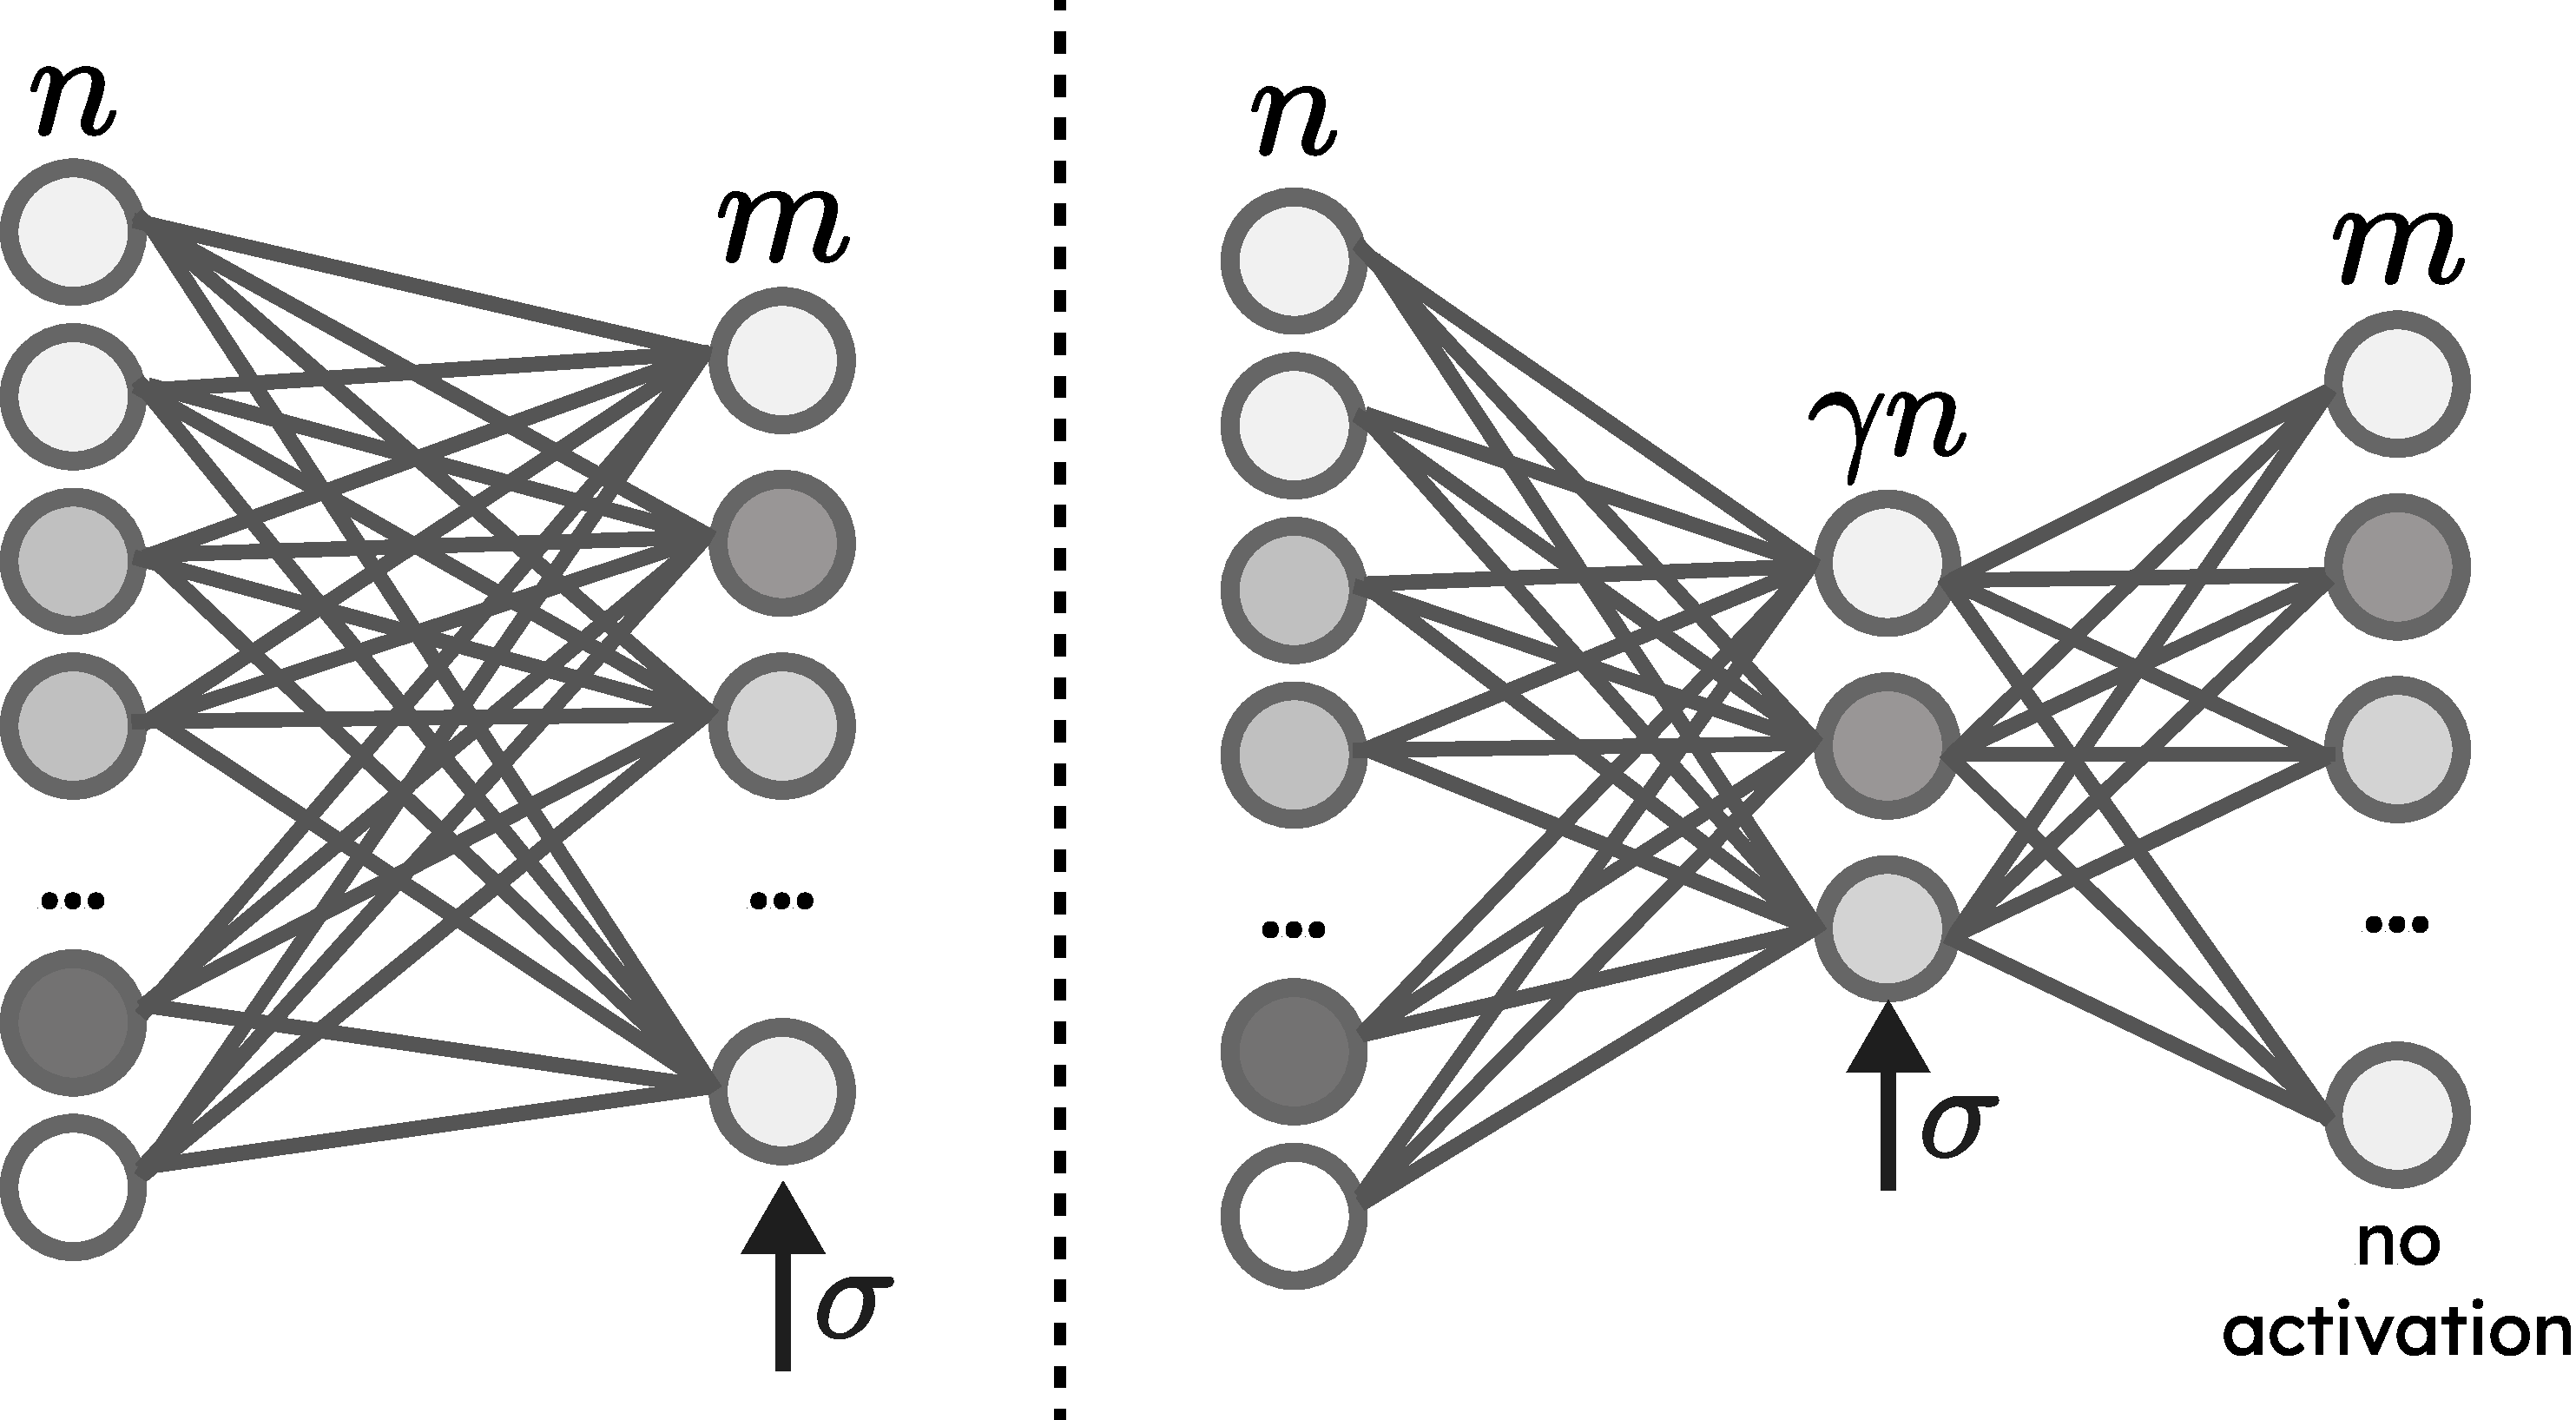
\includegraphics[width=0.7\textwidth]{figures/ed.pdf}
    \caption{The Encoder-Decoder layer.}
    \label{figure:encoder-decoder}
\end{figure}

Why does it help? Consider the following proposition.
\begin{proposition}
    The complexity of the forward pass in the neural network with the
    Encoder-Decoder layer is $\mathcal{O}(h(n + m + \ell))$ multiplications and additions.
\end{proposition}

\textbf{Proof.} The first step is to compute the matrix-vector multiplication
$E\mathbf{x}$, which costs $\mathcal{O}(nh)$ multiplications and additions.
Then, the activation function $\sigma$ is applied to the output of the Encoder,
which costs $\mathcal{O}(h\ell)$ multiplications and additions. Finally, the
matrix-vector multiplication $D(E\mathbf{x})$ costs $\mathcal{O}(\gamma mn)$
multiplications and additions. The total cost is $\mathcal{O}(nh+h\ell+hm)$.
$\blacksquare$

It is not immediately clear why the Encoder-Decoder architecture is beneficial.
Let us consider the concrete example.

\begin{example}
    Припустимо, що $n = 1000$, $m = 10000$, а $h = 10$. Нехай розмірність поля
дорівнює $b = 254$. Тоді складність прямого проходу через нейронну мережу з
одним шаром становить: $10000(1000+254) \approx 107$.

множень і додавань.

Натомість складність прямого проходу через нейронну мережу з шаром Encoder-Decoder дорівнює:
10(1000+10000+254)≈105
10(1000+10000+254)≈105

множень і додавань.

Це дає зменшення в 100 разів, що є суттєвим!
\end{example}

\textbf{Intuition.} Without accounting for the activations, the boost in terms
of number of operations is $\frac{mn}{h(m+n)}$. In particular,
for $n=m$, the boost is $n/2h$, while for $m \gg n$, the boost is roughly $n/h$.
Since we typically want to have $h \ll n$, this results in the significant
boost. This is the reason why the Encoder-Decoder architecture is beneficial for
the large neural networks.

However, due to the fact that we have much less activations in the
Encoder-Decoder architecture, we expect the accuracy to be lower. But how much
lower? This is the primary goal of our next section where we conduct the
experiments to assess the accuracy of the Encoder-Decoder architecture under
various ``squeezing'' factors. Formally, we define the following factor of 
squeezing.

\begin{definition}
    \textbf{Activation Squeezing Factor} $\gamma$ is defined as the ratio of
    activations in the Encoder-Decoder architecture to the number of activations
    in the neural network with the single regular layer. Following the notation
    in this section, we have $\gamma = h/m$.
\end{definition}

\section{Experiment}

We consider the Fashion-MNIST dataset \cite{fashion-mnist}, which consists of
$60000$ RGB images of size $28 \times 28$ pixels. Similarly to the classical
MNIST, this dataset consists of $10$ classes. Example images from the dataset
can be seen in \Cref{figure:mnist}. The primary reason why we employ this 
dataset instead of the classical MNIST is that the latter is too simple and 
thus the results are much less interesting.

\begin{figure}
    \centering
    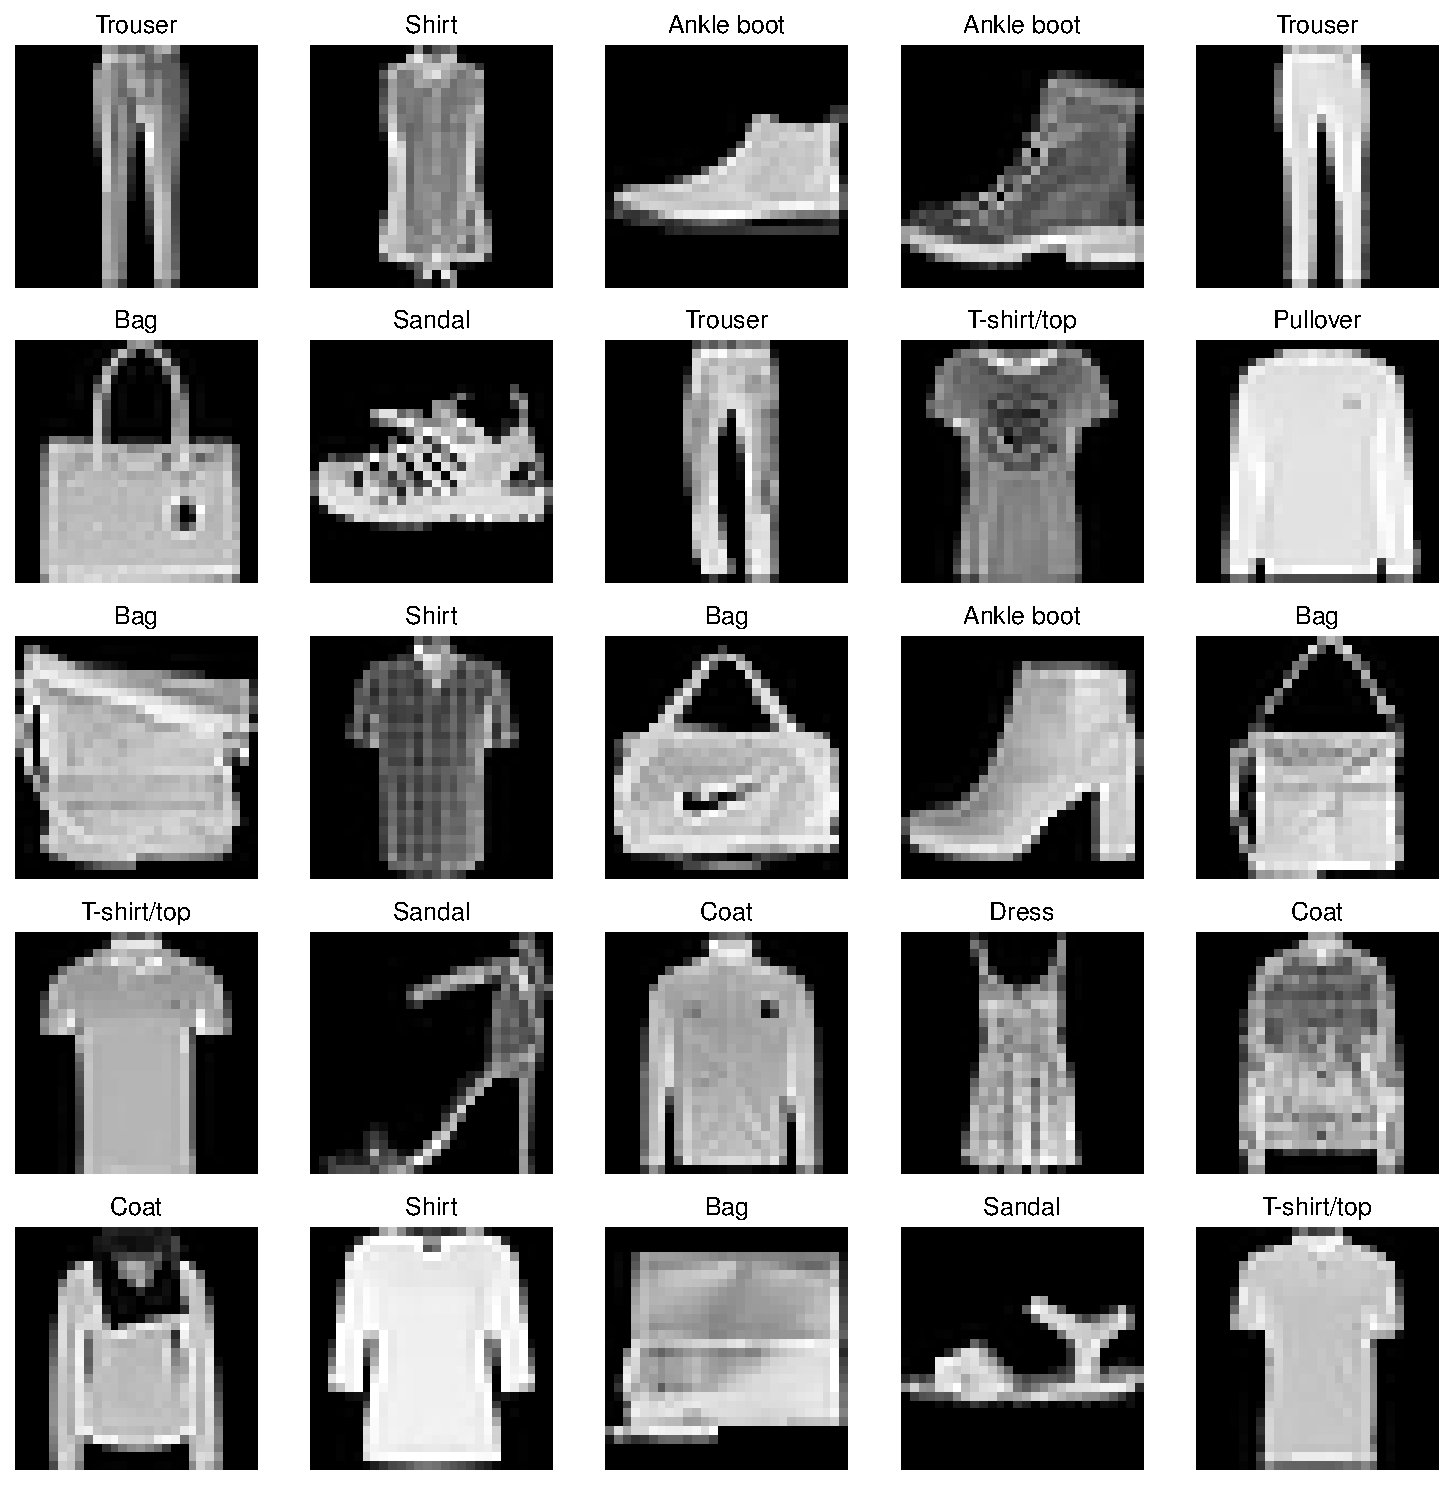
\includegraphics[width=0.7\textwidth]{../code/images/fashion_mnist_grid.pdf}
    \caption{Example images from the Fashion-MNIST dataset \cite{fashion-mnist}.}
    \label{figure:mnist}
\end{figure}

We consider the neural network with the Encoder-Decoder layer with $28 \cdot 28
= 784$ neurons in the input, connected with the Encoder-Decoder layer with
varying parameter $h$ (number of hidden neurons). Namely, the Python (TensorFlow
\cite{tf}) code to construct the Encoder-Decoder layer is provided below:

\begin{minted}{python}
def ed_model(hidden_units: int) -> tf.keras.models.Model:
    return tf.keras.models.Sequential([
        tf.keras.layers.Input(shape=(28,28,1)),
        tf.keras.layers.Flatten(),
        tf.keras.layers.Dense(hidden_units, activation=None),
        tf.keras.layers.ReLU(),
        tf.keras.layers.Dense(100, activation=None),
        tf.keras.layers.BatchNormalization(),
        tf.keras.layers.Dense(10, activation='softmax')
    ])
\end{minted}

Then, we train the model for different values of $h$ and evaluate the maximum
achieved accuracy on the test set. We use the SGD optimizer with the 
learning rate $10^{-3}$ and momentum $0.9$. For each $h$, we use 
the batch size of $128$ and train the model for $100$ epochs. The results are
provided in \Cref{figure:results}.

\begin{figure}[H]
    \centering
    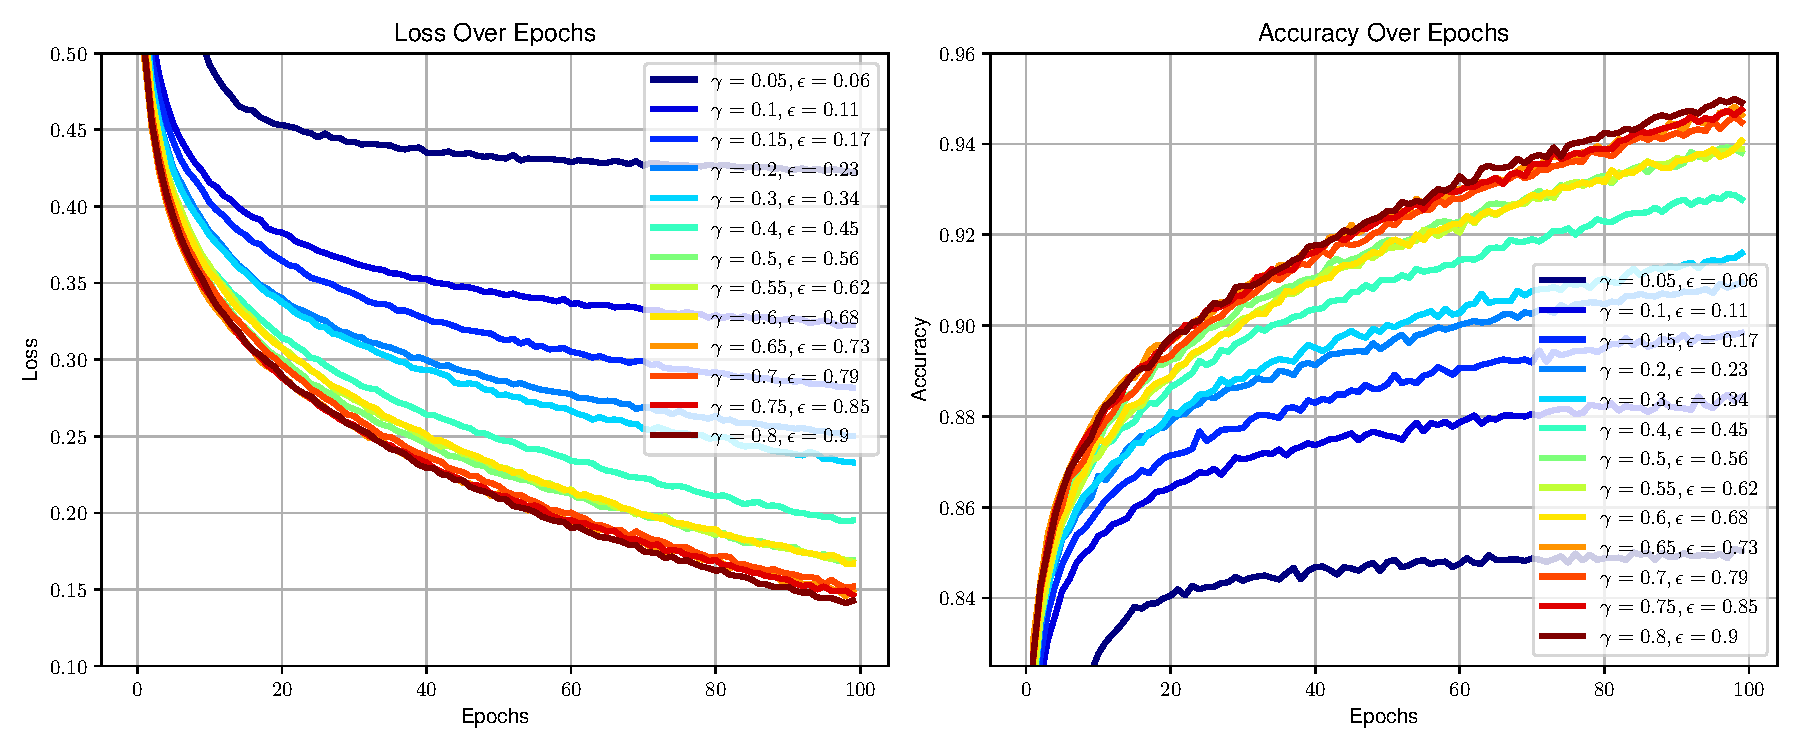
\includegraphics[width=\textwidth]{../code/images/accuracy_loss_over_epochs_3.pdf}
    \caption{Accuracy and loss over epochs for different values of $h$. By 
    $\epsilon$ we denote the ratio of new number of parameters in the model 
    to the original number of parameters.}
    \label{figure:results}
\end{figure}

As can be seen, as expected, the decrease in the number of activations
(parameter $h$) results in worse accuracy: in fact, the accuracy drops by $10\%$
for $\gamma=0.05$ compared to the best recorded accuracy (which is 95\%).
However, very solid results can still be obtained using relatively small values
of $\gamma$: namely, for $\gamma=0.3$ the accuracy is close to 92\%. We 
additionally depict the dependence of max accuracy on the parameter $\gamma$, 
which is specified in \Cref{fig:accuracies}.

\begin{figure}
    \centering
    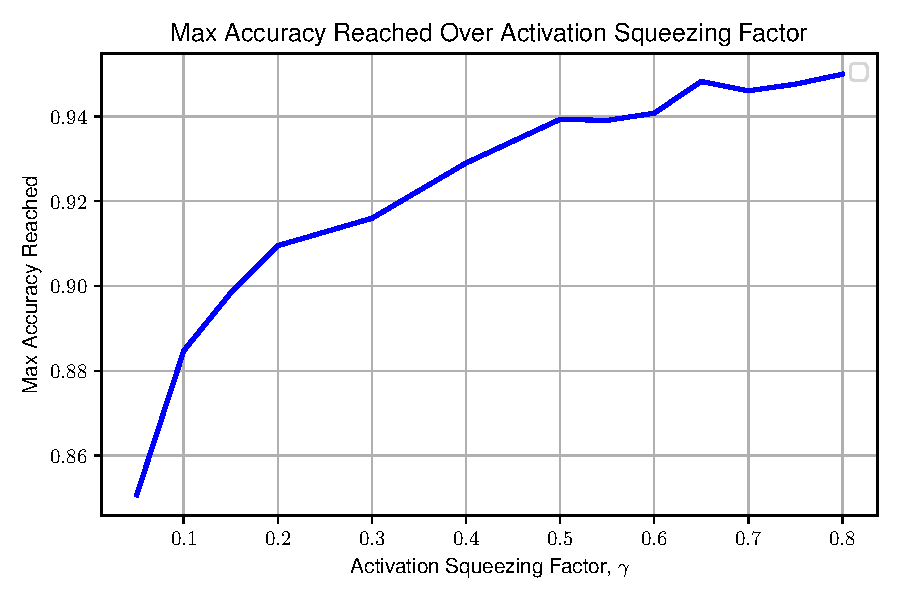
\includegraphics[width=0.8\textwidth]{../code/images/max_accuracy_over_squeeze.pdf}
    \caption{The dependence of max accuracy on the parameter $\gamma$.}
    \label{fig:accuracies}
\end{figure}

This way, we can indeed reduce the number of activations in the neural network, 
subsequently reducing the number of operations in the arithmetical circuit by 
sacrifising a non-significant amount of accuracy. This is the main result of our paper.

\subsection{Future Work}

Note that we presented the substitution only for the fully-connected layers. The
next step is to extend the results to the convolutional layers. One of the
examples of such activation-friendly convolutional layers is the so-called
Squeeze-and-Excitation layer, presented by \cite{se-network}, see
\Cref{figure:se} for illustration. Given input volume $\mathbf{X} \in
\mathbb{R}^{W \times H \times C}$ (where $C$ is the number of channels and $W
\times H$ is the image size), we first apply the Global Average Pooling to
extract the channel-wise average values $\mathbf{z} \in \mathbb{R}^C$. Then,
$\mathbf{z}$ is passed through the Encoder-Decoder Layer with the scaling vector
$\mathbf{s} \in \mathbb{R}^C$ as the output. Finally, each image
$\mathbf{X}_{[:,:,i]}$ gets multiplied by the corresponding scaling factor $s_i$
for $i \in [C]$. The main advantage of this layer is that it is very lightweight
and can be used in the arithmetical circuits since all the non-linear operations
are conducted in the Encoder-Decoder layer, which is only $C$ neurons wide.

\begin{figure}
    \centering
    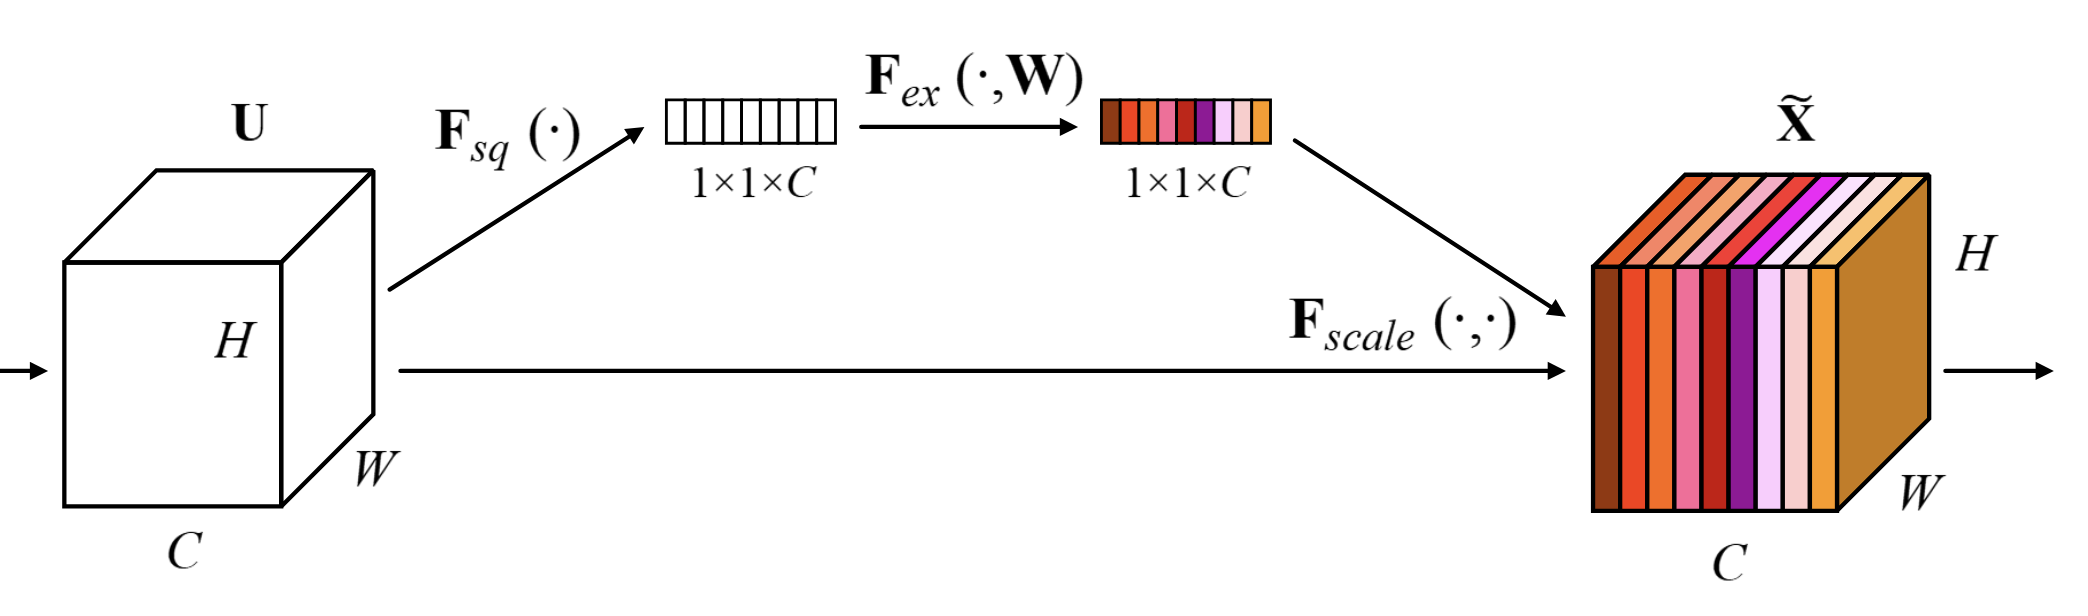
\includegraphics[width=\textwidth]{figures/se.png}
    \caption{The Squeeze-and-Excitation layer. Figure taken from 
    the original paper \cite{se-network}.}
    \label{figure:se}
\end{figure}

The natural question arising is whether we can figure out more
activation-friendly layers in the context of Convolutional Neural Networks or,
possibly, in Recurrent Neural Networks and Large Language Models.

Finally, more experiments are needed to fully understand the balance between the
accuracy and the number of activations. In particular, we would like to
understand the trade-off between the number of activations and the accuracy for
the different datasets.

\section{Conclusion}\label{section:conclusion}

In this paper, we introduced the notion of activation-friendly neural networks
and explained the wide range of applications where they can be used. We
proceeded to show that the Encoder-Decoder architecture can be used to reduce
the number of activations in the neural network, while keeping the accuracy
relatively high. We conducted the experiments on the Fashion-MNIST dataset and
showed that the accuracy drops by only $2\%$ when both the number of activations
and parameters is reduced by more than $3$ times. We also provided the
theoretical foundation for the Encoder-Decoder architecture and showed that it
is indeed beneficial in terms of the number of operations in the arithmetical
circuit. Finally, we discussed the future work and the possible extensions of
the results to the convolutional layers and other types of neural networks.

% --- References ---
\bibliographystyle{alpha} 
\bibliography{refs} 

\end{document}
